\documentclass{article}
\usepackage{tikz}
\usepackage{amsmath}

\begin{document}

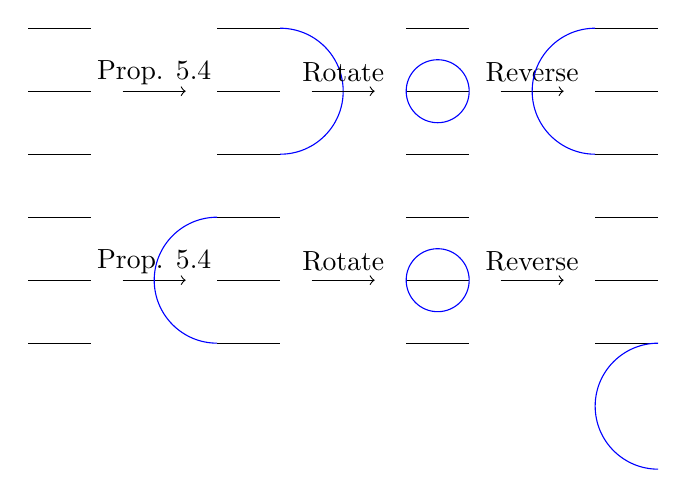
\begin{tikzpicture}[scale=0.8]
% First row - first diagram
\draw[black] (0,0) -- (1,0);
\draw[black] (0,1) -- (1,1);
\draw[black] (0,2) -- (1,2);

% First row - arrow and label
\draw[->] (1.5,1) -- (2.5,1);
\node at (2,1.3) {Prop. 5.4};

% First row - second diagram
\draw[black] (3,0) -- (4,0);
\draw[black] (3,1) -- (4,1);
\draw[black] (3,2) -- (4,2);
\draw[blue] (4,0) arc (-90:90:1);

% First row - arrow and label
\draw[->] (4.5,1) -- (5.5,1);
\node at (5,1.3) {Rotate};

% First row - third diagram
\draw[black] (6,0) -- (7,0);
\draw[black] (6,1) -- (7,1);
\draw[black] (6,2) -- (7,2);
\draw[blue] (7,1) arc (0:180:0.5);
\draw[blue] (7,1) arc (0:-180:0.5);

% First row - arrow and label
\draw[->] (7.5,1) -- (8.5,1);
\node at (8,1.3) {Reverse};

% First row - fourth diagram
\draw[black] (9,0) -- (10,0);
\draw[black] (9,1) -- (10,1);
\draw[black] (9,2) -- (10,2);
\draw[blue] (9,0) arc (270:90:1);

% Second row - first diagram
\draw[black] (0,-1) -- (1,-1);
\draw[black] (0,-2) -- (1,-2);
\draw[black] (0,-3) -- (1,-3);

% Second row - arrow and label
\draw[->] (1.5,-2) -- (2.5,-2);
\node at (2,-1.7) {Prop. 5.4};

% Second row - second diagram
\draw[black] (3,-1) -- (4,-1);
\draw[black] (3,-2) -- (4,-2);
\draw[black] (3,-3) -- (4,-3);
\draw[blue] (3,-3) arc (270:90:1);

% Second row - arrow and label
\draw[->] (4.5,-2) -- (5.5,-2);
\node at (5,-1.7) {Rotate};

% Second row - third diagram
\draw[black] (6,-1) -- (7,-1);
\draw[black] (6,-2) -- (7,-2);
\draw[black] (6,-3) -- (7,-3);
\draw[blue] (6,-2) arc (180:0:0.5);
\draw[blue] (6,-2) arc (180:360:0.5);

% Second row - arrow and label
\draw[->] (7.5,-2) -- (8.5,-2);
\node at (8,-1.7) {Reverse};

% Second row - fourth diagram
\draw[black] (9,-1) -- (10,-1);
\draw[black] (9,-2) -- (10,-2);
\draw[black] (9,-3) -- (10,-3);
\draw[blue] (10,-3) arc (90:270:1);

\end{tikzpicture}

\end{document}